% !TEX options=--shell-escape

\documentclass{report}
\usepackage[T1]{fontenc}
\usepackage{lmodern}

\usepackage{titlesec}
\usepackage{hyperref}
\usepackage{nameref}

\usepackage[a4paper, margin=2.5cm, headsep=0pt]{geometry}

\usepackage{tgadventor}
\renewcommand{\familydefault}{\sfdefault}

\usepackage{graphicx}
\usepackage{subcaption}
\usepackage{titlepic}
\usepackage[skip=5pt]{caption}

\usepackage[ddmmyyyy]{datetime}
\usepackage[section]{placeins}
\usepackage{enumitem}

\usepackage{minted}
\usepackage[dvipsnames]{xcolor}

\definecolor{bg}{gray}{0.1}

\titleformat{\chapter}{\normalfont\huge}{\bf\thechapter.}{20pt}{\huge\bf}
\titlespacing{\chapter}{0pt}{12pt plus 4pt minus 2pt}{8pt plus 2pt minus 2pt}

\hypersetup{
  colorlinks,
  citecolor=black,
  filecolor=black,
  linkcolor=black,
  urlcolor=blue
}

\graphicspath{technisch verslag imgs/}

\usemintedstyle{monokai}

\newdate{creation}{02}{02}{2022}

\begin{document}
\begin{titlepage}
\centering
\vfill
\bfseries\Huge{Pacenstein\\\large{- Technisch Verslag -}}\\
\normalfont\normalsize\displaydate{creation}
\vfill

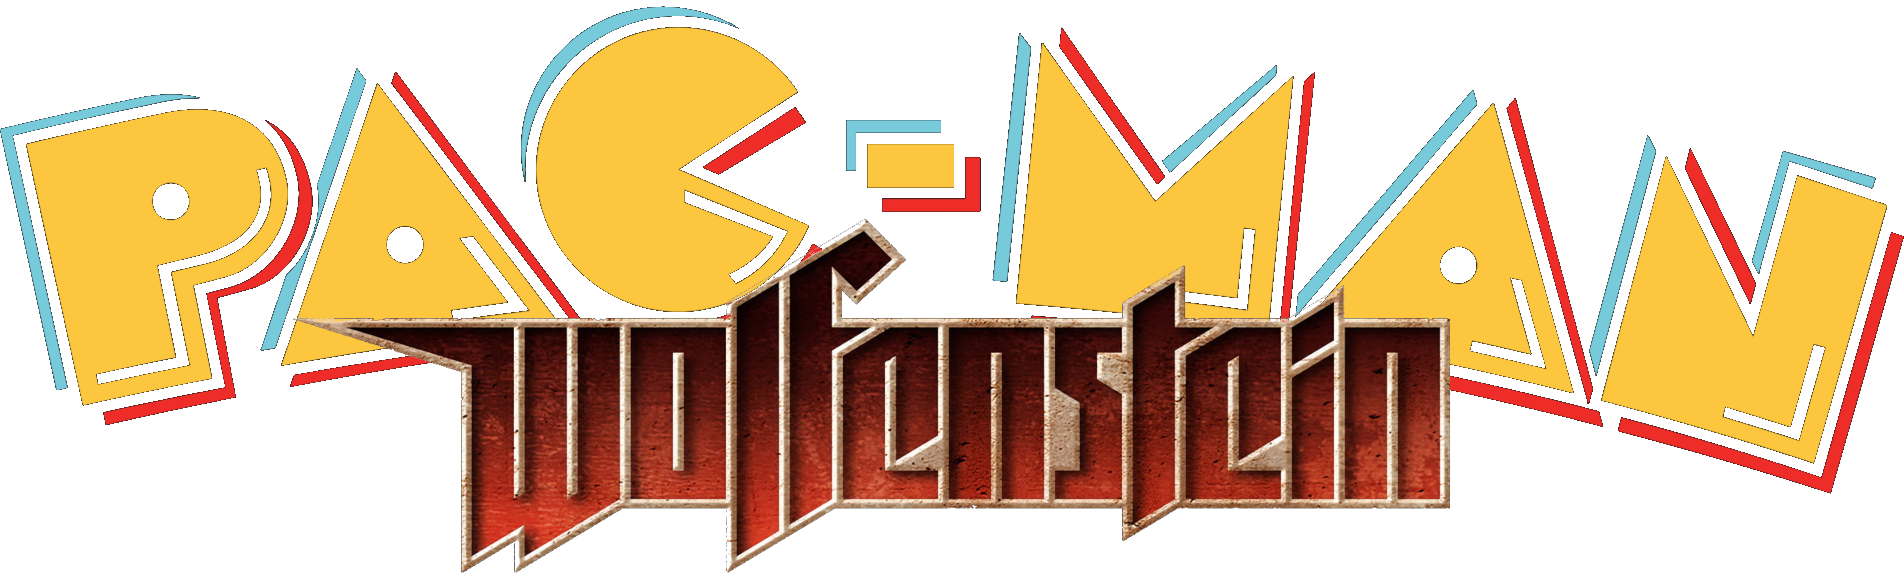
\includegraphics[width=\textwidth]{../res/pacenstein.png}
\vfill
\large{
  Lennard Duinkerken\\
  Emma Raijmakers\\
  Daan Roth\\
  Jarno Bröcker
}
\vfill
\end{titlepage}

\tableofcontents

\chapter{Inleiding} % (fold)
\label{cha:inleiding}
In dit document leggen wij uit hoe onze game werkt op technisch gebied. Complexe of onduidelijke, en de meest belangrijke delen uit de code worden toegelicht in een poging te verduidelijken wat er gebeurd.

In het klassendiagram is snel terug te zien hoe de classes tot elkaar verhouden en welke methods en members ertoe behoren. Raycasting, het meest complexe deel van dit project, gebruiken wij om 2D te vertalen naar 3D. De input manager, asset manager en state machine vormen de backbone van de game. Alles gerelateerd aan afbeeldingen, inputs en outputs wordt uiteindelijk door die drie classes beheerd.

We hebben ook een overzicht gemaakt van alle states waar onze game zich in kan bevinden. Van elk van deze states is een korte beschrijving van diens functie, en op welk moment tijdens het spelen deze aan bod zal komen.

Voor alle entities, items, ghosts, de player, en zo voort... is een omschrijving te vinden. Zo zijn ghosts items, de player is een entity, en items zijn ook entities.

Als laatste is er een overzicht van alle textures, afbeeldingen, sprites, en alle andere dingen die niet source code zijn, met een bijbehorende beschrijving natuurlijk.

\section{Klassendiagram} % (fold)
\label{sec:klassendiagram}
Om weer te geven hoe de classes samenhangen binnen dit project hebben wij een klassendiagram geproduceerd.
\begin{figure}[h]
  \centering
  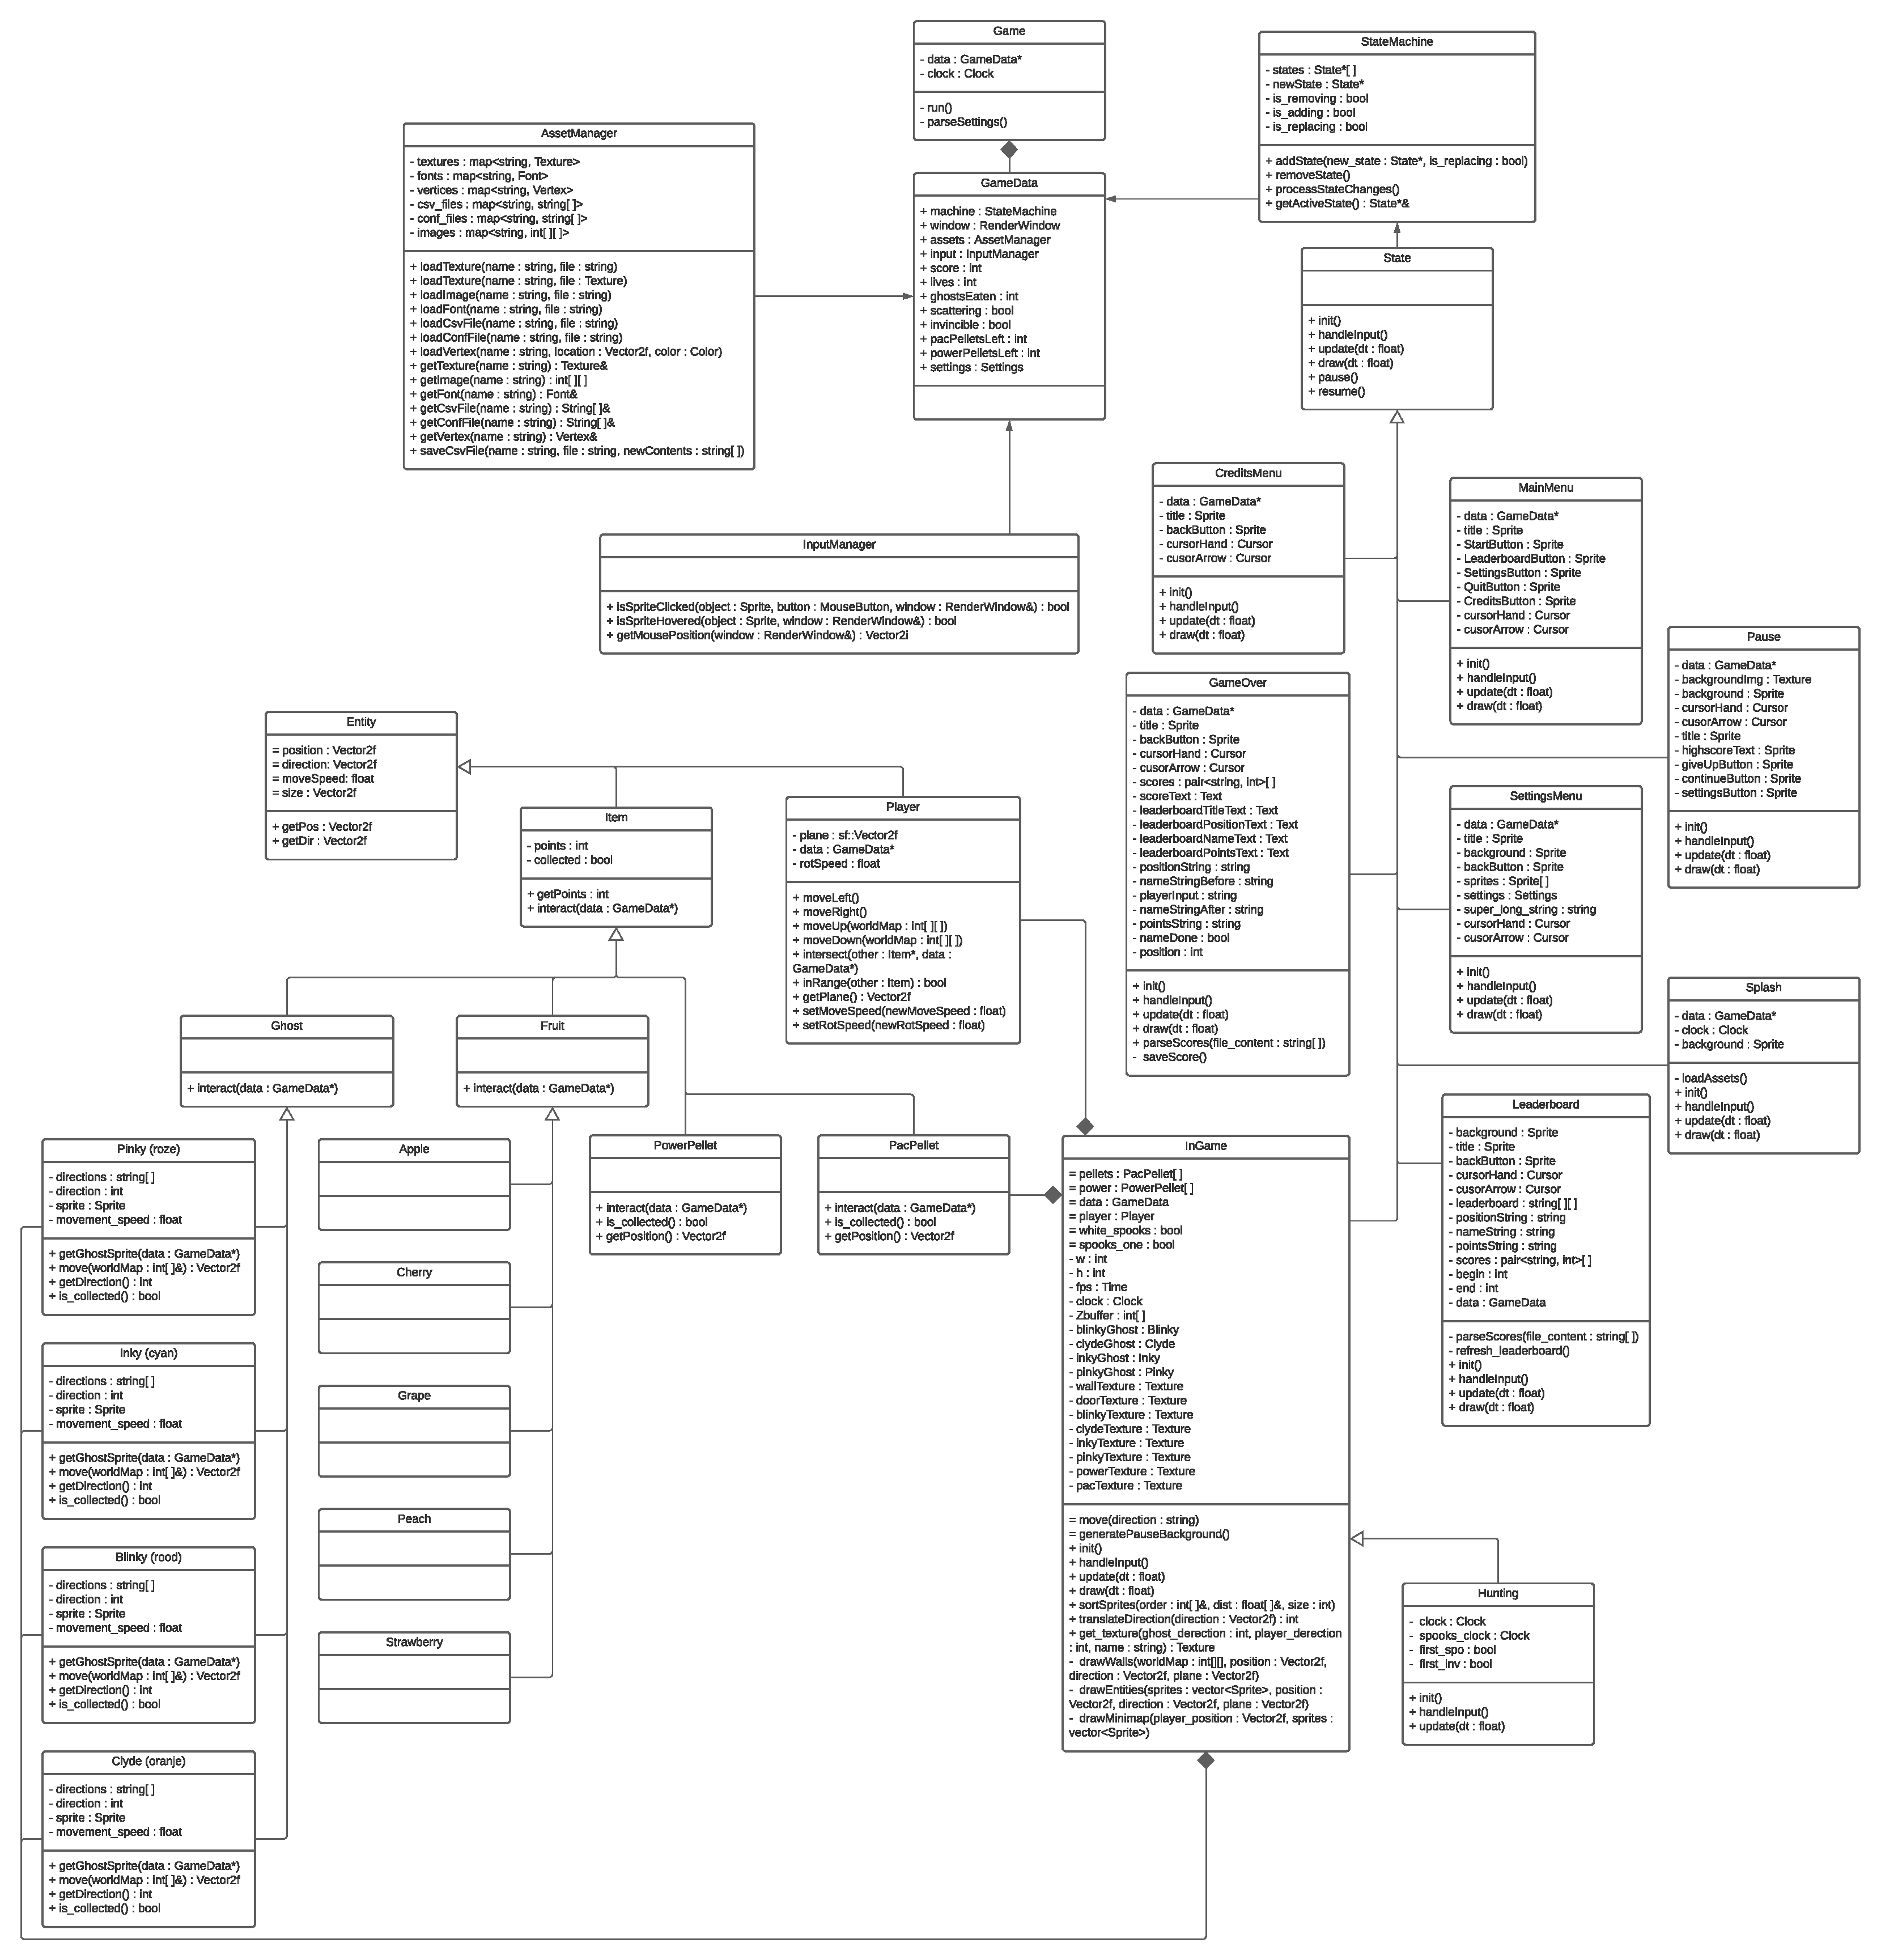
\includegraphics[width=.73\textwidth]{THGA Pacenstein - Class_Object Diagram.pdf}
  \caption{File: \url{THGA Pacenstein - Class_Object Diagram.pdf}\\(klik om originele bestand te zien, of zoom in)}
\end{figure}
% section klassendiagram (end)
% chapter inleiding (end)

\chapter{Game Engine} % (fold)
\label{cha:game_engine}

  \section{Raycasting} % (fold)
  \label{sec:raycasting}
    \subsection{Waarom Raycasting} % (fold)
    \label{sub:waarom_raycasting}
    Dit project gebruikt raycasting om een 2d wereld, op het scherm er uit te laten zien als een 3d wereld. Raycasting is hiervoor gebruikt omdat het een relatief simpele methode is om de wereld 3d te maken. Dit project gebruikt geen hardware acceleratie, dus het is belangrijk dat het een lichte simpele methode is. Vandaar de keuze voor raycasting.
    \begin{figure}[h]
      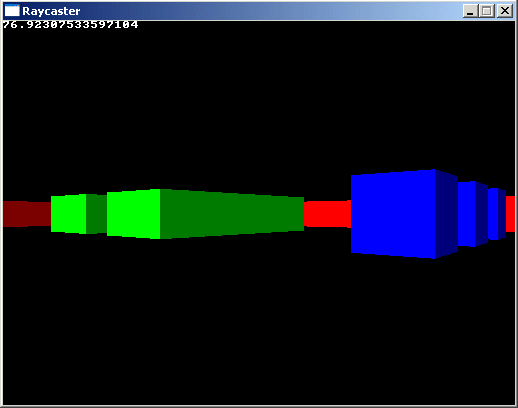
\includegraphics[width=\textwidth]{technisch verslag imgs/raycasteruntextured.png}
      \caption{Source: \url{https://lodev.org/cgtutor/raycasting.html}}
    \end{figure}
    % subsection waarom_raycasting (end)

    \subsection{Hoe werkt Raycasing - In het kort} % (fold)
    \label{sub:hoe_werkt_raycasing_in_het_kort}
    Raycasting is een erg snel process, en kan op heel low end hardware draaien. Denk aan de originele wolfenstein of doom.
    De player schiet voor elke pixel van het scherm in de breedte, een ray uit. Hij cast dus een ray. Deze ray moet een eindje reizen vaak. Wanneer deze een muur raakt, zal hij kijken hoe ver hij heeft moeten reizen. Hij gebruikt deze afstand om op het scherm een lijn te trekken. Deze lijn kan groter en kleiner worden gemaakt gebaseerd op de afstand. Wanneer dit process herhaald wordt voor elke pixel, zal er een muur zichtbaar moeten zijn.

    Dit is de raycaster in een notendop, en een erge versimpeling. Bij de goed werkende raycaster komt veel meer kijken. Heb je de muur van voren geraakt? Of heb je de muur aan de zijkant geraakt? Kan je dit gebruiken om een nep schaduw op een van de kanten te zetten zodat je het verschil ziet tussen de muren?
    % subsection hoe_werkt_raycasing_in_het_kort (end)

    \subsection{Hoe werkt Raycasting - In het lang} % (fold)
    \label{sub:hoe_werkt_raycasting_in_het_lang}
    Hiervoor is \url{https://lodev.org/cgtutor/raycasting.html} een goede bron met uitleg. Deze website loopt stap voor stap af hoe een raycaster gemaakt moet worden. En enkele optimalisaties. De raycaster van de game is gebaseerd op hoofdstuk 1 en 3.
    % subsection hoe_werkt_raycasting_in_het_lang (end)

    \subsection{Port en Origineel} % (fold)
    \label{sub:port_en_origineel}
    De raycaster van de engine is een directe port van \url{https://lodev.org/cgtutor/raycasting.html}. De comments van de originele broncode zijn er bij gehouden, en variabelen hebben dezelfde naam waar dit mogelijk is.

    Het grootste verschil tussen de port en het origineel is het feit dat het origineel SDL gebruikt, en de port SFML. Ook is de code wat aangepast zodat deze meer volgens de C++ standaarden werkt. Bijvoorbeeld de c-arrays waar de map is in opgeslagen zijn veranderd in \mintinline[bgcolor=bg]{c++}|std::array|.

    De raycaster is opgedeelt in 2 losse raycasters. 1 voor de muren, en 1 voor de entities.
    De raycaster voor de entities heeft de meeste veranderingen gekregen vergeleken met het origineel in verband met SFML. Deze 2 raycasters worden in de \mintinline[bgcolor=bg]{c++}|InGameState.cpp| en \mintinline[bgcolor=bg]{c++}|InGameState.hpp| gemaakt en uitgevoerd. Dit gebeurt in de draw functie.
    % subsection port_en_origineel (end)

    \subsection{Grote Verschillen} % (fold)
    \label{sub:grote_verschillen}

    \subsubsection{Movement} % (fold)
    \label{ssub:movement}

\textbf{Origineel}
\begin{minted}[bgcolor=bg, fontsize=\footnotesize, linenos]{c++}
readKeys();
if (keyDown(SDLK_UP)) {
  if(worldMap[int(posX + dirX * moveSpeed)][int(posY)] == false) posX += dirX * moveSpeed;
  if(worldMap[int(posX)][int(posY + dirY * moveSpeed)] == false) posY += dirY * moveSpeed;
}
if (keyDown(SDLK_DOWN)) {
  if(worldMap[int(posX - dirX * moveSpeed)][int(posY)] == false) posX -= dirX * moveSpeed;
  if(worldMap[int(posX)][int(posY - dirY * moveSpeed)] == false) posY -= dirY * moveSpeed;
}
//rotate to the right
if (keyDown(SDLK_RIGHT)) {
  double oldDirX = dirX;
  dirX = dirX * cos(-rotSpeed) - dirY * sin(-rotSpeed);
  dirY = oldDirX * sin(-rotSpeed) + dirY * cos(-rotSpeed);
  double oldPlaneX = planeX;
  planeX = planeX * cos(-rotSpeed) - planeY * sin(-rotSpeed);
  planeY = oldPlaneX * sin(-rotSpeed) + planeY * cos(-rotSpeed);
}
//rotate to the left
if (keyDown(SDLK_LEFT)) {
  double oldDirX = dirX;
  dirX = dirX * cos(rotSpeed) - dirY * sin(rotSpeed);
  dirY = oldDirX * sin(rotSpeed) + dirY * cos(rotSpeed);
  double oldPlaneX = planeX;
  planeX = planeX * cos(rotSpeed) - planeY * sin(rotSpeed);
  planeY = oldPlaneX * sin(rotSpeed) + planeY * cos(rotSpeed);
}
\end{minted}
\newpage
\textbf{Port}
\begin{minted}[bgcolor=bg, fontsize=\footnotesize, linenos]{c++}
sf::Event event;

while (this->data->window.pollEvent(event)) {
  this->data->window.setMouseCursorVisible(false);

  if (sf::Event::Closed == event.type) this->data->window.close();

  if (sf::Keyboard::isKeyPressed(sf::Keyboard::Key::KEY_UP)
  ||  sf::Keyboard::isKeyPressed(sf::Keyboard::Key::KEY_ALT_UP)
  ||  sf::Keyboard::isKeyPressed(sf::Keyboard::Key::KEY_DOWN)
  ||  sf::Keyboard::isKeyPressed(sf::Keyboard::Key::KEY_ALT_DOWN)
  ||  sf::Keyboard::isKeyPressed(sf::Keyboard::Key::KEY_RIGHT)
  ||  sf::Keyboard::isKeyPressed(sf::Keyboard::Key::KEY_ALT_RIGHT)
  ||  sf::Keyboard::isKeyPressed(sf::Keyboard::Key::KEY_LEFT)
  ||  sf::Keyboard::isKeyPressed(sf::Keyboard::Key::KEY_ALT_LEFT)) {
      this->data->machine.addState(state_ref_t(std::make_unique<HuntingState>(this->data)), true);
  }

  if (sf::Keyboard::isKeyPressed(sf::Keyboard::Key::KEY_PAUSE)
  ||  sf::Keyboard::isKeyPressed(sf::Keyboard::Key::KEY_ALT_PAUSE)) {
      this->generatePauseBackground();
      this->data->machine.addState(state_ref_t(std::make_unique<PauseState>(this->data)), false);
  }

  if (sf::Keyboard::isKeyPressed(sf::Keyboard::Key::KEY_EXIT)) {
      this->data->window.close();
  }
}
\end{minted}
      % subsubsection movement (end)

      \subsubsection{Muren tekenen} % (fold)
      \label{ssub:textures_laden}

\textbf{Origineel}
\begin{minted}[bgcolor=bg, fontsize=\footnotesize, linenos]{c++}
if(side == 0) perpWallDist = (sideDistX - deltaDistX);
else          perpWallDist = (sideDistY - deltaDistY);
\end{minted}
\\
\textbf{Port}
\begin{minted}[bgcolor=bg, fontsize=\footnotesize, linenos]{c++}
if (!side) {
  perpWallDist = fabs((mapX - rayPosX + (1 - stepX) / 2) / rayDirX);
  while (rayPosY > 1) {
    rayPosY = -1;
  }
  textureSectionX = rayPosY;
}
else {
  perpWallDist = fabs((mapY - rayPosY + (1 - stepY) / 2) / rayDirY);

while (rayPosX > 1) rayPosX =- 1;
  textureSectionX = rayPosX;
}
\end{minted}
      % subsubsection textures_laden (end)
\newpage
      \subsubsection{Sprites sorteren} % (fold)
      \label{ssub:sprites_sorteren}
\textbf{Origineel}
\begin{minted}[bgcolor=bg, fontsize=\footnotesize, linenos]{c++}
void sortSprites(int* order, double* dist, int amount) {
  std::vector<std::pair<double, int>> sprites(amount);
  for(int i = 0; i < amount; i++) {
    sprites[i].first = dist[i];
    sprites[i].second = order[i];
  }
  std::sort(sprites.begin(), sprites.end());
  for(int i = 0; i < amount; i++) {
    dist[i] = sprites[amount - i - 1].first;
    order[i] = sprites[amount - i - 1].second;
  }
}
\end{minted}
\\
\textbf{Port}
\begin{minted}[bgcolor=bg, fontsize=\footnotesize, linenos]{c++}
void InGameState::sortSprites(std::vector<int> &order, std::vector<float> &dist, int size) {
  std::cout << "Done \n";
  int gap = size;
  bool flag = true;
  while (gap != 1 || flag) {
    gap = (gap * 10) / 13;
    if (gap < 1) gap = 1;
    flag = false;

    for (int i = 0; i < size - gap; i++) {
      int j = i + gap;
      if (dist[i] < dist[j]) {
        std::swap(dist[i],dist[j]);
        std::swap(order[i],order[j]);
        flag = true;
      }
    }
  }
}
\end{minted}
      % subsubsection sprites_sorteren (end)

      \subsubsection{Sprites tekenen} % (fold)
      \label{ssub:sprites_tekenen}
\textbf{Origineel}
\begin{minted}[bgcolor=bg, fontsize=\footnotesize, linenos]{c++}
//loop through every vertical stripe of the sprite on screen
for(int stripe = drawStartX; stripe < drawEndX; stripe++) {
  int texX = int(256 * (stripe - (-spriteWidth / 2 + spriteScreenX)) * texWidth / spriteWidth) / 256;

  //the conditions in the if are:
  //1) it's in front of camera plane so you don't see things behind you
  //2) it's on the screen (left)
  //3) it's on the screen (right)
  //4) ZBuffer, with perpendicular distance

  if(transformY > 0 && stripe > 0 && stripe < w && transformY < ZBuffer[stripe]) {
    for(int y = drawStartY; y < drawEndY; y++) { //for every pixel of the current stripe

      //256 and 128 factors to avoid floats
      int d = (y-vMoveScreen) * 256 - h * 128 + spriteHeight * 128;
      int texY = ((d * texHeight) / spriteHeight) / 256;

      //get current color from the texture
      Uint32 color = texture[sprite[spriteOrder[i]].texture][texWidth * texY + texX];

      //paint pixel if it isn't black, black is the invisible color
      if((color & 0x00FFFFFF) != 0) buffer[y][stripe] = color;
    }
  }
}

\end{minted}
\\
\textbf{Port}
\begin{minted}[bgcolor=bg, fontsize=\footnotesize, linenos]{c++}
//loop through every vertical stripe of the sprite on screen
for (int stripe = drawStartX; stripe <= drawEndX; ++stripe) {
  if (stripe < 0) {
    drawStartX += 1;
    continue;
  }
  // are other walls in front
  if (transformY > this->ZBuffer[stripe]) {
    drawStartX += 1;
    continue;
  }
  break;
}

int newWidth = drawEndX - drawStartX;
float d = (float)drawWidth / (float)newWidth;

spriteLeft = texture_width - (float)texture_width / d;

for (int stripe = drawEndX; stripe > drawStartX; --stripe) {
  if (stripe > width) {
    drawEndX -= 1;
    continue;
  }
  if (transformY > this->ZBuffer[stripe]) {
    drawEndX -= 1;
    continue;
  }
  break; // y break, de continues snap ik, maar deze is niet nodig
}

newWidth = drawEndX - drawOrigStartX;
d = (float)drawWidth / (float)newWidth;

spriteRight = (float)texture_width / d;

sf::VertexArray spriteQuad(sf::Quads, 4);

spriteQuad[0].position  = sf::Vector2f(drawStartX,  drawStartY);
spriteQuad[0].texCoords = sf::Vector2f(spriteLeft,  spriteTop);
spriteQuad[1].position  = sf::Vector2f(drawEndX,    drawStartY);
spriteQuad[1].texCoords = sf::Vector2f(spriteRight, spriteTop);
spriteQuad[2].position  = sf::Vector2f(drawEndX,    drawEndY);
spriteQuad[2].texCoords = sf::Vector2f(spriteRight, spriteBottom);
spriteQuad[3].position  = sf::Vector2f(drawStartX,  drawEndY);
spriteQuad[3].texCoords = sf::Vector2f(spriteLeft,  spriteBottom);

this->data->window.draw(spriteQuad, &sprite.tex);
\end{minted}
      % subsubsection sprites_tekenen (end)
    % subsection grote_verschillen (end)
  % section raycasting (end)

  \section{Game Logic} % (fold)
  \label{sec:game_logic}

    \subsection{Player Movement} % (fold)
    \label{sub:player_movement}
    De Player class is gebaseerd op de Entity, en heeft daarom \mintinline[bgcolor=bg]{c++}|sf::Vector2f|’s om zijn position en direction op te slaan.
    \subsubsection{Entity.hpp} % (fold)
    \label{ssub:entity_hpp}

    \begin{minted}[bgcolor=bg, fontsize=\footnotesize, linenos]{c++}
protected:
  sf::Vector2f position, direction, size;
  float moveSpeed;
};
    \end{minted}
    % subsubsection entity_hpp (end)
    Deze wordt door de player input aangepast met zijn input, de handleInput functie. Deze veranderd de state met de juiste waarden.
    \subsubsection{InGameState.hpp} % (fold)
    \label{ssub:ingamestate_hpp}

    \begin{minted}[bgcolor=bg, fontsize=\footnotesize, linenos]{c++}
void InGameState::handleInput() {
  sf::Event event;

  while (this->data->window.pollEvent(event)) {
    this->data->window.setMouseCursorVisible(false);

    if (sf::Event::Closed == event.type) this->data->window.close();

    if (sf::Keyboard::isKeyPressed(sf::Keyboard::Key::KEY_UP)
    ||  sf::Keyboard::isKeyPressed(sf::Keyboard::Key::KEY_ALT_UP)
    ||  sf::Keyboard::isKeyPressed(sf::Keyboard::Key::KEY_DOWN)
    ||  sf::Keyboard::isKeyPressed(sf::Keyboard::Key::KEY_ALT_DOWN)
    ||  sf::Keyboard::isKeyPressed(sf::Keyboard::Key::KEY_RIGHT)
    ||  sf::Keyboard::isKeyPressed(sf::Keyboard::Key::KEY_ALT_RIGHT)
    ||  sf::Keyboard::isKeyPressed(sf::Keyboard::Key::KEY_LEFT)
    ||  sf::Keyboard::isKeyPressed(sf::Keyboard::Key::KEY_ALT_LEFT)) {
      this->data->machine.addState(state_ref_t(std::make_unique<HuntingState>(this->data)), true);
    }

    if (sf::Keyboard::isKeyPressed(sf::Keyboard::Key::KEY_PAUSE)
    ||  sf::Keyboard::isKeyPressed(sf::Keyboard::Key::KEY_ALT_PAUSE)) {
      this->generatePauseBackground();
      this->data->machine.addState(state_ref_t(std::make_unique<PauseState>(this->data)), false);
    }

    if (sf::Keyboard::isKeyPressed(sf::Keyboard::Key::KEY_EXIT)) {
      this->data->window.close();
    }
  }
}
    \end{minted}
    % subsubsection ingamestate_hpp (end)
    % subsection player_movement (end)

    \subsection{Player Interaction} % (fold)
    \label{sub:player_interaction}
    De player kan met andere Items in de game interacteren. Dit wordt gedaan door de volgende functie:
    \begin{minted}[bgcolor=bg, fontsize=\footnotesize, linenos]{c++}
bool Player::intersect(Item & other, game_data_ref_t data){
  bool collision = int(this->position.x) == int(other.getPos().x)
    && int(this->position.y) == int(other.getPos().y);
  if (collision) other.interact(this->data);
  return collision;
}
    \end{minted}

    In deze functie wordt gecheckt of de speler op hetzelfde block van de map staat als het meegegeven item. Als dit het geval is, dan is er een collision. Als er een collision is dan wordt de interact functie van het Item waar de speler mee collide aangeroepen. In deze interact functie wordt verder afgehandeld wat er gebeurd bij de collision met een bepaald Item.
    \begin{minted}[bgcolor=bg, fontsize=\footnotesize, linenos]{c++}
void PowerPellet::interact(game_data_ref_t data) {
  data->powerPelletsLeft--;
  collected = true;
  data->score += points;
  data->scattering = true;
}
    \end{minted}
    Een voorbeeld van een interact functie is de interact functie van de PowerPellet class. Hierin wordt aangegeven dat de pellet is verzameld, de score is verhoogd en scattering (als de speler de ghosts kan opeten) actief is.

    De interact functie is een abstracte functie van de Item class, waar alle items van erven. Hierdoor wordt het voor iedere class die erft van een Item, en dus ook als item in het spel voor kan komen, verplicht om aan te geven hoe het interact met de player.
    % subsection player_interaction (end)

    \subsection{Ghost Movement} % (fold)
    \label{sub:ghost_movement}
    De movement van de ghosts is zo geïmplementeerd dat het per ghost kan verschillen. De Ghost class heeft een abstracte move functie, zodat iedere ghost zijn eigen movement moet regelen. Een voorbeeld is de move functie van de Blinky class:
    \begin{minted}[bgcolor=bg, fontsize=\footnotesize, linenos]{c++}
sf::Vector2f Blinky::move(const map_t & worldMap){
  switch (this->direction) {
    case 1: // Noord
      if((this->position.y - int(this->position.y)) < 0.5){
        if(worldMap[int(this->position.x)][int(this->position.y) - 1] == 3) {
          //if block above ghost is a wall
          this->direction = rand() % 4 + 1;
          break;
        }
      }
      this->position = {this->position.x, this->position.y - movement_speed};
    break;

    case 2: // Oost
      if((this->position.x - int(this->position.x)) < 0.5){
        if(worldMap[int(this->position.x) - 1][int(this->position.y)] == 3) {
          //if block left of ghost is a wall
          this->direction = rand() % 4 + 1;
          break;
        }
      }
      this->position = {this->position.x - movement_speed, this->position.y};
    break;

    case 3: // Zuid
      if((this->position.y - int(this->position.y)) > 0.5){
        if(worldMap[int(this->position.x)][int(this->position.y) + 1] == 3) {
          //if block below ghost is a wall
          this->direction = rand() % 4 + 1;
          break;
        }
      }
      this->position = {this->position.x, this->position.y + movement_speed};
    break;

    case 4: // West
      if((this->position.x - int(this->position.x)) > 0.5){
        if(worldMap[int(this->position.x) + 1][int(this->position.y)] == 3) {
          //if block right of ghost is a wall
          this->direction = rand() % 4 + 1;
          break;
        }
      }
      this->position = {this->position.x + movement_speed, this->position.y};
    break;
  }
  return this->position;
}
    \end{minted}
    De functie berekent de nieuwe positie van Blinky als een \mintinline[bgcolor=bg]{c++}|sf::Vector2f|. Dit wordt gedaan door de richting die Blinky op gaat te gebruiken. Er wordt gekeken of Blinky in dezelfde richting door kan gaan of dat er een muur voor hem staat. Als er een muur staat, wordt de richting van Blinky aangepast naar een random nieuwe richting. De nieuwe positie van Blinky wordt berekend door de movement speed op de juiste manier op te tellen bij de oude positie. Deze nieuwe positie wordt teruggegeven.
    % subsection ghost_movement (end)

    \subsection{Optimalisatie} % (fold)
    \label{sub:optimalisatie}
    In de game is optimalisatie toegepast door middel van de inRange functie in de Player class. In deze functie wordt gekeken of de positie van een Item binnen een vierkant van grootte 5 om de speler valt. Als dit het geval is, wordt er true teruggegeven en anders false.
    \begin{minted}[bgcolor=bg, fontsize=\footnotesize, linenos]{c++}
bool Player::inRange(Item & other){
  sf::RectangleShape playerRect;
  playerRect.setPosition(sf::Vector2f(this->position.x - 5, this->position.y - 5));
  playerRect.setSize(sf::Vector2f(10.0, 10.0));
  return playerRect.getGlobalBounds().contains(other.getPos());
}
    \end{minted}
    De returnwaarde van deze functie wordt gebruikt bij het tekenen van de Pac en Power Pellets. De pellets worden alleen op de map weergegeven als ze in de range van de speler zitten. Dit zorgt ervoor dat er meer pellets aan de map toegevoegd kunnen worden zonder dat dit de performance verminderd.
    % subsection optimalisatie (end)
  % section game_logic (end)

  \section{Asset Manager} % (fold)
  \label{sec:asset_manager}
  De asset manager is verantwoordelijk voor het beheren van de textures, map, fonts, afbeeldingen, configuratiebestand, leaderboard bestand en SFML vertices.

  De map wordt ingeladen van een .png-bestand. Deze wordt door de asset manager omgezet naar een vector van vectoren. Door middel van de verschillende kleuren pixels zullen de vectoren hun waarden krijgen. In deze vectoren staat aangegeven op welke locatie welke muur geschreven moet worden. Deze wordt ingeladen door de \mintinline[bgcolor=bg]{c++}|assetManager::loadImage| functie.

  De configuratie van de game staat in een settings.conf bestand. Deze wordt ingeladen door de \mintinline[bgcolor=bg]{c++}|assetManager::getConfFile| functie.

  Het leaderboard wordt ingeladen door de \mintinline[bgcolor=bg]{c++}|assetManager::loadCsvFile| functie, en geeft deze een naam voor gemakkelijk gebruik.

  De textures worden ingeladen door de \mintinline[bgcolor=bg]{c++}|assetManager::loadTexture| functie.

  De fonts worden ingeladen door de \mintinline[bgcolor=bg]{c++}|assetManager::loadFonts| functie.

  De SFML vertexes worden ingeladen door \mintinline[bgcolor=bg]{c++}|assetManager::loadVertex|.

  De afbeeldingen worden ingeladen en gegeven door de \mintinline[bgcolor=bg]{c++}|assetManager::getImage| function. Deze wordt teruggegeven in een map met de naam en de image zelf.
  % section asset_manager (end)

  \section{Input Manager} % (fold)
  \label{sec:input_manager}
  De input manager houdt de positie van de muiscursor bij en controleert of sprites aangeklikt zijn. Een aantal van onze sprites werken namelijk als knoppen in de menus.
  % section input_manager (end)

  \section{State Machine} % (fold)
  \label{sec:state_machine}
  De state machine beheert de states door ze op een stack te zetten. De bovenste state is altijd de actieve state. Wanneer een state toegevoegd wordt komt deze bovenop te staan en wordt deze dus ook actief.

  Het is mogelijk een state toe te voegen en die state de huidige actieve state laten vervangen. Het vervangen van een state is nuttig wanneer je niet terug wilt gaan naar de huidige state. Als hij niet vervangen wordt, dan kun je de bovenste state verwijderen om terug te keren naar de vorige state.

  De state machine is in staat om states te pauzeren en te laten vervolgen en gaat daar mee bezig wanneer \mintinline[bgcolor=bg]{c++}|stateMachine::processStateChange| aangeroepen wordt.
  Het is ook mogelijk om de huidige actieve state op te vragen via \mintinline[bgcolor=bg]{c++}|stateMachine::getActiveState|.
  % section state_machine (end)
% chapter game_engine (end)

\chapter{States} % (fold)
\label{cha:states}
De states worden gebruikt om tussen verschillende delen van de game te switchen. Dit wordt gedaan door een state op de stack van de State Machine te zetten of hem er weer af te halen. Iedere state heeft zijn eigen functionaliteiten en graphical interface die in de volgende hoofdstukken verder worden uitgelegd.

  \section{Splash} % (fold)
  \label{sec:splash}
  De Splash State wordt gebruikt om alle afbeeldingen die gebruikt worden in de game te laden als Textures. De afbeeldingen worden door de Asset Manager opgeslagen en kunnen in de rest van de game gebruikt worden, zonder dat ze opnieuw geladen moeten worden.
  \begin{figure}[!ht]
    \centering
    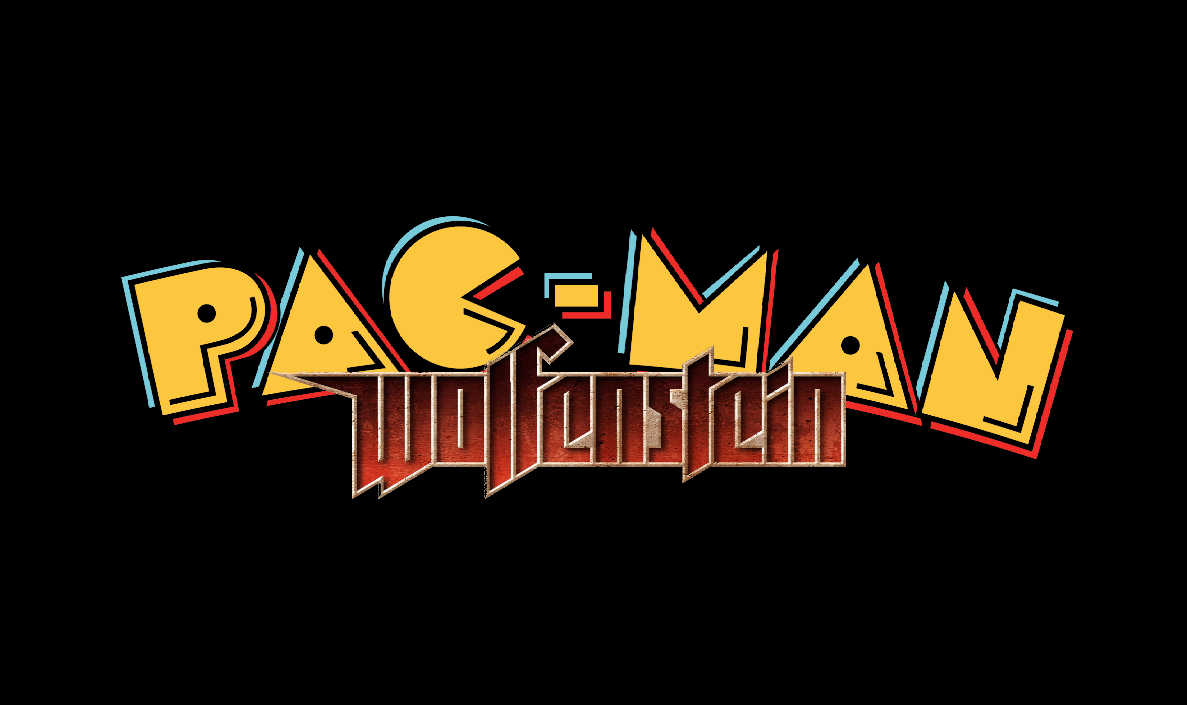
\includegraphics[width=.95\textwidth]{technisch verslag imgs/splash.png}
    \caption{Het splash screen - Toont het logo terwijl het assets laadt.}
  \end{figure}
  % section splash (end)

  \section{Menu's} % (fold)
  \label{sec:menu_s}
  De game Pacenstein heeft verschillende menus die informatie aan de speler laten zien. De menus beschikken over tekstelementen en knoppen. Knoppen zijn klikbare objecten die de speler doorsturen naar andere states. De muis van de speler veranderd in een wijzende muis als er over een knop wordt gehoverd.

    \subsection{Main Menu} % (fold)
    \label{sub:main_menu}
    Het Main Menu is het menu dat de speler krijgt te zien na de Splash State. In dit menu zijn verschillende keuzemogelijkheden te zien. Dit zijn de knoppen Start Game, Leaderboard, Settings, Quit Game en Credits. Als de speler op de knop Start Game klikt, wordt de game gestart. Leaderboard laat de vorige scores zien. Settings laat de controls van de game zien, Quit Game sluit de game af en Credits (de ronde knop met het vraagteken) laat de makers van de game zien.
    \begin{figure}[!ht]
      \centering
      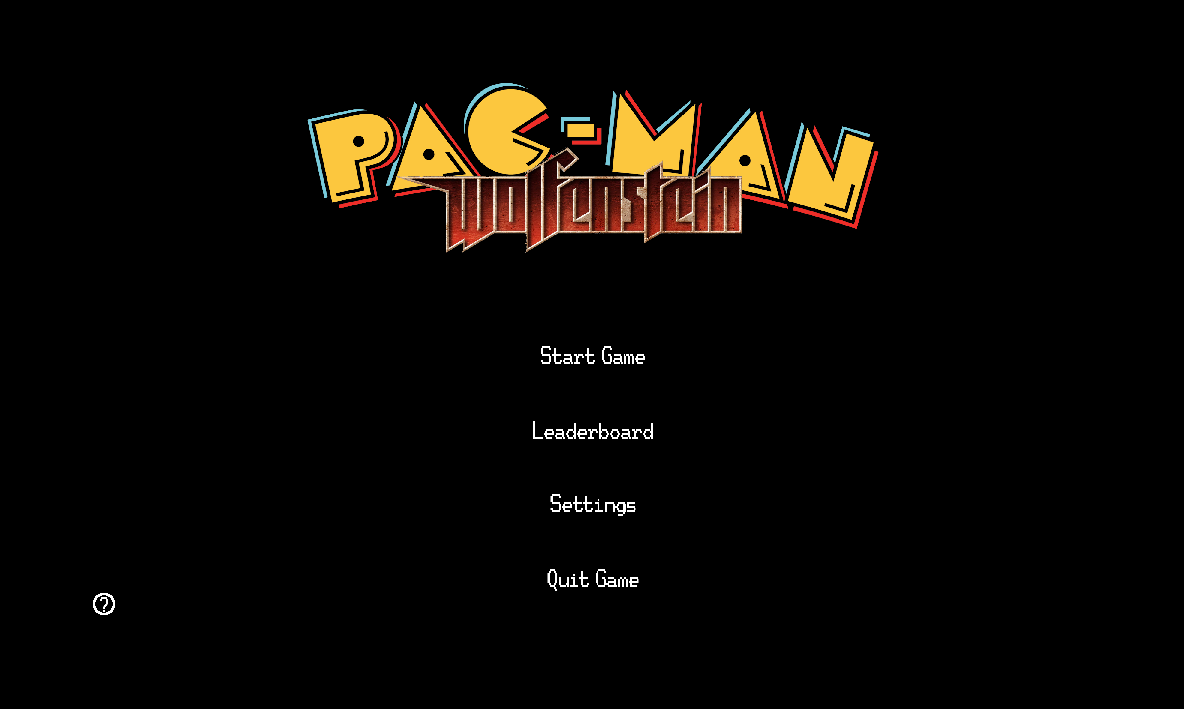
\includegraphics[width=.95\textwidth]{technisch verslag imgs/main.png}
      \caption{Het main menu - Begin het spel, bekijk het leaderboard, en meer.}
    \end{figure}
    % subsection main_menu (end)

    \subsection{Settings Menu} % (fold)
    \label{sub:settings_menu}
    Het Settings Menu laat de verschillende controls zien die de speler kan gebruiken tijdens de game. De speler kan bewegen door middel van WASD en de pijltjestoetsen. Verder is de game te pauzeren door op de escape knop te drukken en af te sluiten door op de delete knop te drukken. De Back knop linksboven gaat terug naar het vorige menu.
    \begin{figure}[!ht]
      \centering
      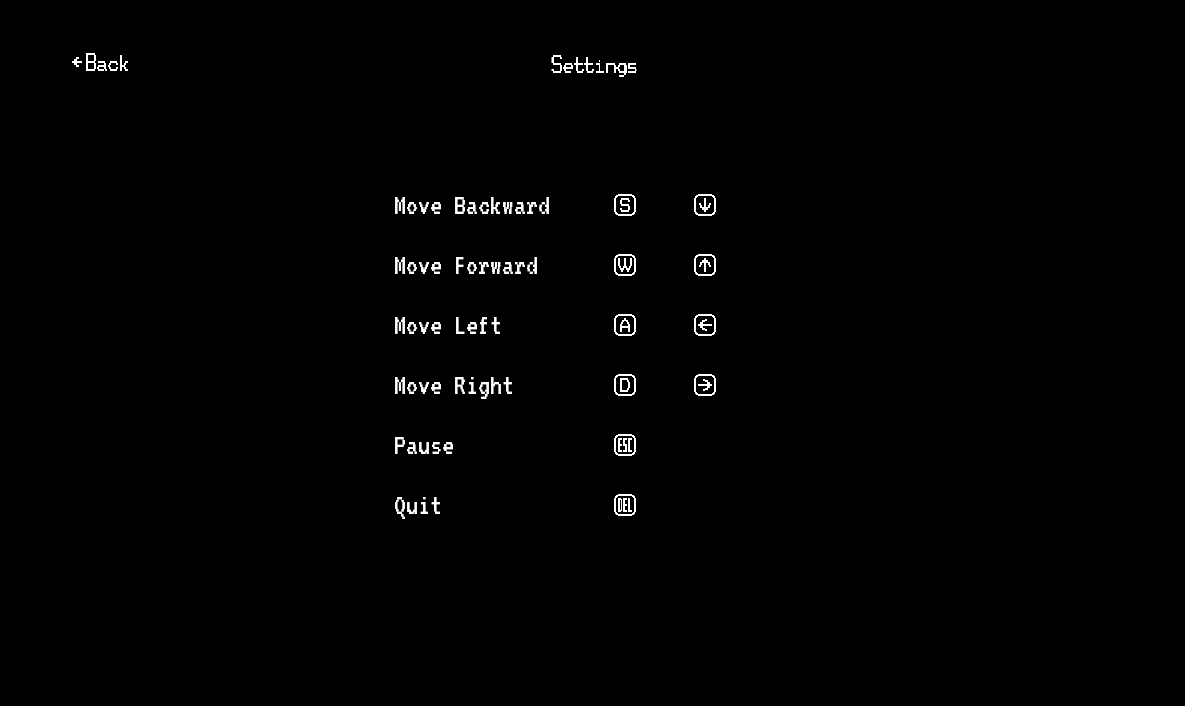
\includegraphics[width=.95\textwidth]{technisch verslag imgs/settings.png}
      \caption{Het settings menu - Hier kun je de keybindings bekijken.}
    \end{figure}
    % subsection settings_menu (end)

    \subsection{Leaderboard Menu} % (fold)
    \label{sub:leaderboard_menu}
    Het Leaderboard Menu laat de scores van de voorgaande spelers zien op een aflopende volgorde. Ook is de naam van de voorgaande spelers bij de bijhorende score te zien. De Back knop linksboven gaat terug naar het hoofdmenu.
    \begin{figure}[!ht]
      \centering
      
\includegraphics[width=.95\textwidth]{technisch verslag imgs/leaderboard.png}
      \caption{Het leaderboard - Hier staan alle scores op een rij.}
    \end{figure}
    % subsection leaderboard_menu (end)

    \subsection{Credits Menu} % (fold)
    \label{sub:credits_menu}
    Het Credits Menu laat de makers van de game zien. Verder gaat de Back Button weer terug naar het Main Menu.
    \begin{figure}[!ht]
      \centering
      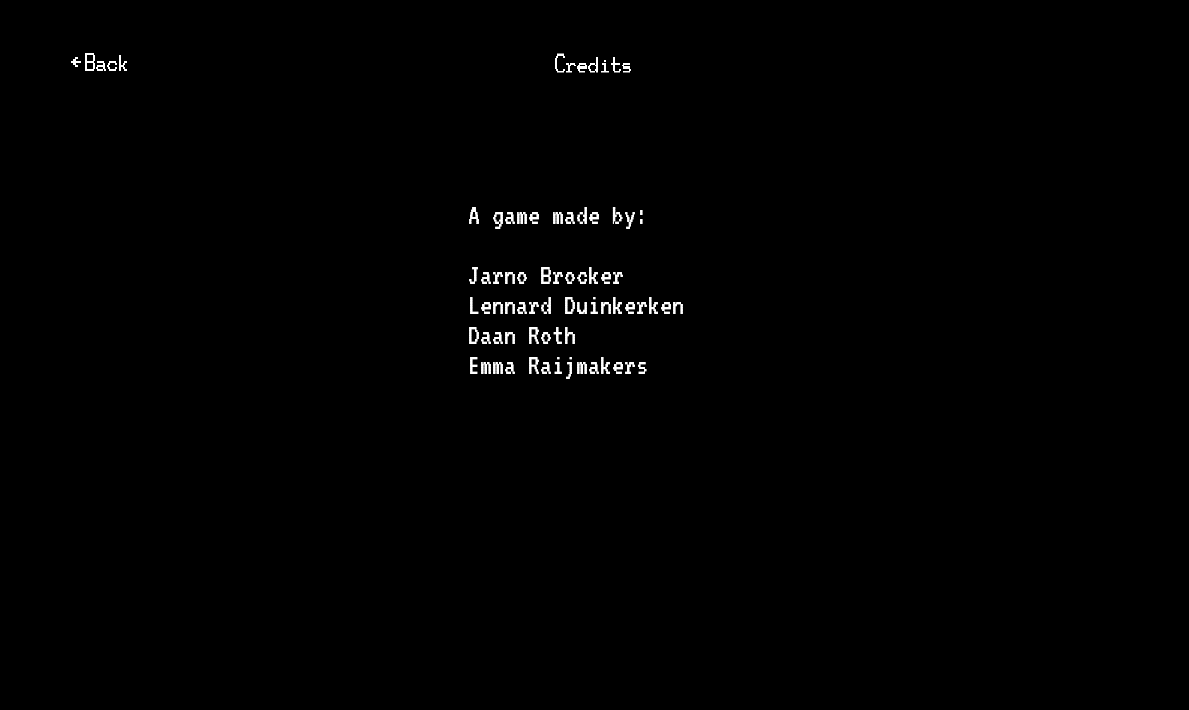
\includegraphics[width=.95\textwidth]{technisch verslag imgs/credits.png}
      \caption{De credits - Dit zijn de mensen die aan het spel gewerkt hebben.}
    \end{figure}
    % subsection credits_menu (end)
  % section menu_s (end)

  \section{In Game} % (fold)
  \label{sec:in_game}
  De In Game State is de state waarin de gameplay begint. In deze state worden de Ghosts, Pacpellets en PowerPellets op hun posities gezet en wordt de map met alle entities door middel van Raycasting getekend. Als de speler begint met bewegen, wordt de state veranderd naar de Hunting State. De logica van de gameplay is te vinden in het hoofdstuk Game Logic.
  % section in_game (end)

  \section{Hunting} % (fold)
  \label{sec:hunting}
  In de Hunting State kan de speler Pacpellets en Powerpellets verzamelen voor een hogere score. Pacpellets geven 10 punten Powerpellets 100 punten. Als een Powerpellet is opgepakt kan de speler de spoken opeten. Het eerste spook dat wordt opgegeten geeft 200 punten de tweede 400, de derde 800 en de laatste 1600. Een speler kan ook levens verliezen als hij aangeraakt wordt door een spook. Als de speler zijn 3 levens verliest of als alle Pacpellets en Powerpellets zijn verzameld, is het spel afgelopen. De state gaat dan naar de Game Over State.
  \begin{figure}[h]
      \centering
      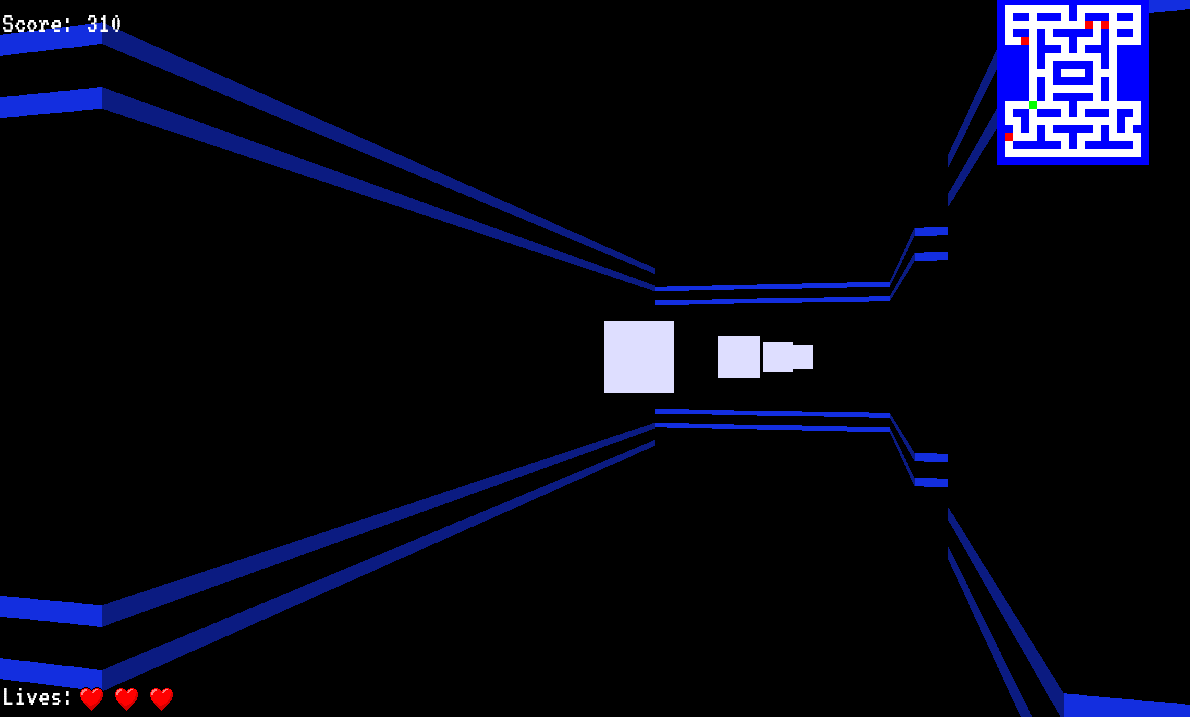
\includegraphics[width=.95\textwidth]{technisch verslag imgs/hunting.png}
      \caption{In game, hunting - Het spel is bezig en je wordt achterna gezeten.}
    \end{figure}
  % section hunting (end)

  \section{Pause State} % (fold)
  \label{sec:pause_state}
  De speler kan tijdens de gameplay op Escape drukken om in de Pause State te komen. De Pause State wordt gebruikt om de game te pauzeren. In de Pause State zijn de knoppen Give Up, Continue en Settings te vinden. Give Up zorgt ervoor dat de speler naar de \nameref{sec:game_over} state gaat, Continue zorgt ervoor dat de game verder gaat en Settings gaat naar de \nameref{sub:settings_menu} State.
  \begin{figure}[h]
      \centering
      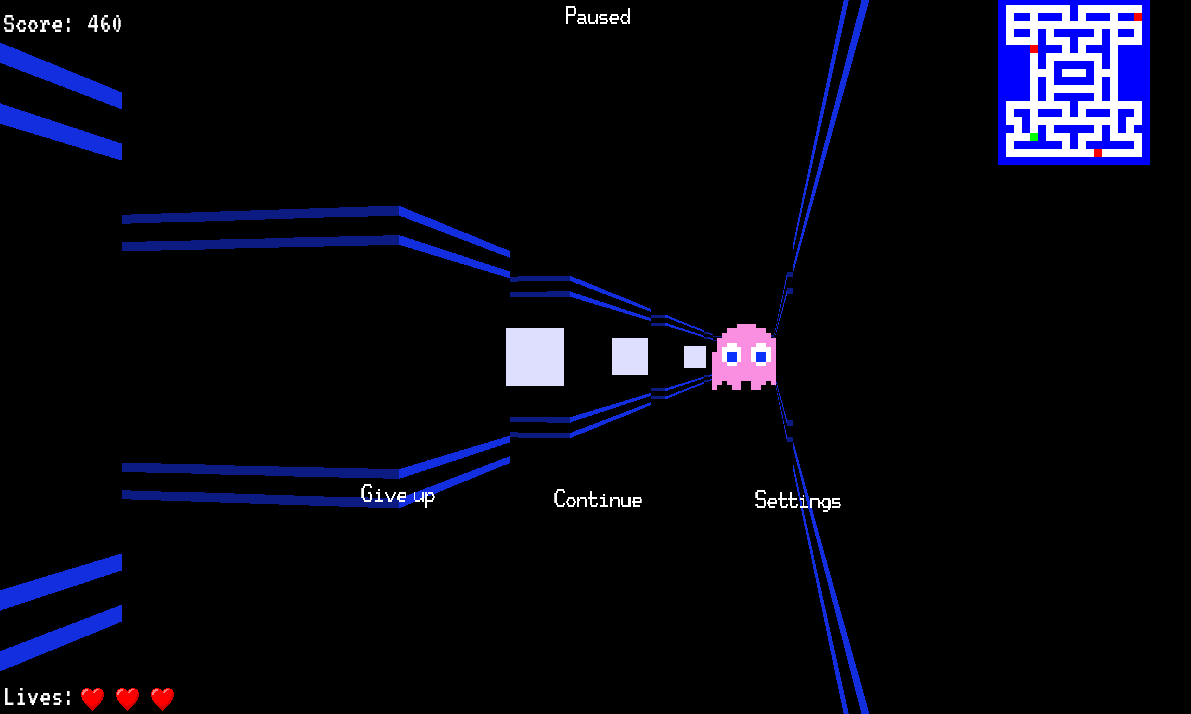
\includegraphics[width=.95\textwidth]{technisch verslag imgs/pause.png}
      \caption{Het pauze menu - Het spel is gepauzeerd.}
    \end{figure}
  % section pause_state (end)

  \section{Game Over} % (fold)
  \label{sec:game_over}
  De Game Over State is te zien als het spel is afgelopen of als de speler opgeeft. In de Game Over State is het leaderboard te zien van voorgaande scores. De score die de huidige speler heeft behaald wordt op de juiste plek in het leaderboard gezet. De speler kan vervolgens een naam invoeren bij zijn behaalde score. Door op enter te drukken wordt de score opgeslagen. Er is ook een knop, To Main Menu, om terug te gaan naar het Main Menu.
  \begin{figure}[h]
      \centering
      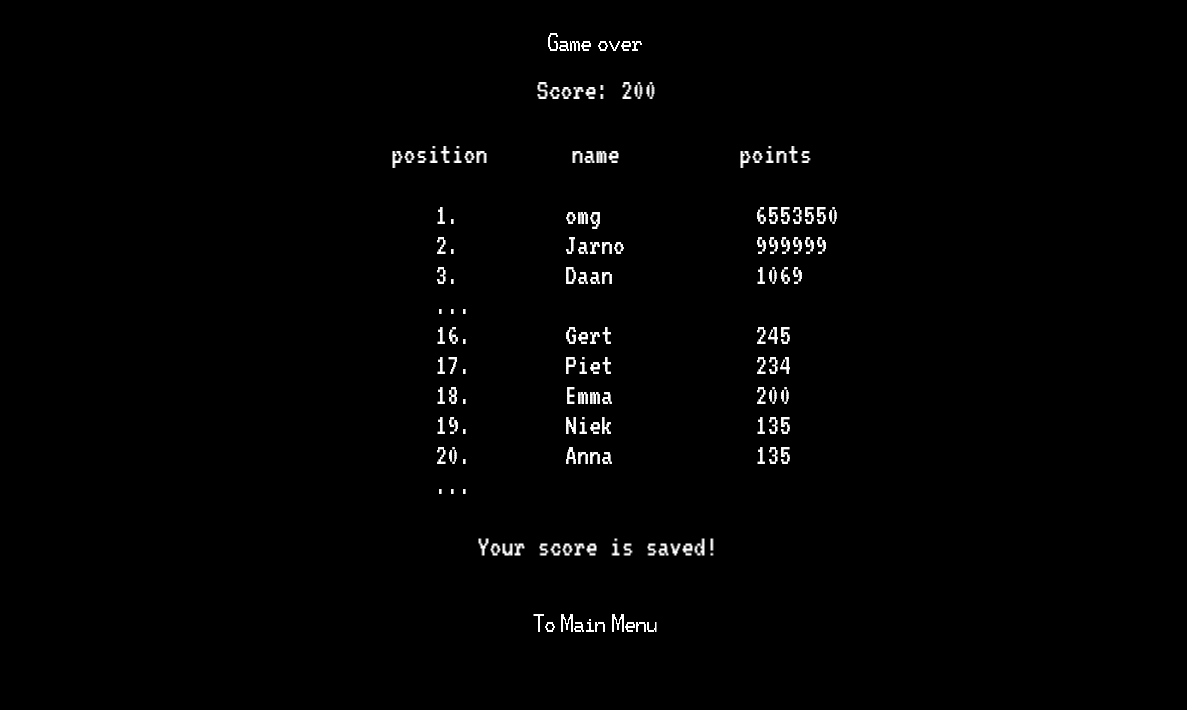
\includegraphics[width=\textwidth]{technisch verslag imgs/game over.png}
      \caption{Game over - Het einde van het spel waar je je score kunt vastleggen.}
    \end{figure}
  % section game_over (end)
% chapter states (end)

\chapter{Entities} % (fold)
\label{cha:entities}
Entities zijn alle objecten die gebruikt worden tijdens de gameplay. Dit zijn de Player, de Ghosts en de te verzamelen objecten: Pacpellets en Powerpellets.

  \section{Items} % (fold)
  \label{sec:items}
  Onder items vallen alle entities behalve de speler. Een Item is een object dat interactie kan hebben met de speler.

    \subsection{Fruits} % (fold)
    \label{sub:fruits}
    Fruits zijn Items die op een random positie op de map spawnen. De speler kan Fruits verzamelen voor meer punten. De Fruits zijn: Apple, Cherry, Grape, Peach en Strawberry en ieder Fruit heeft zijn eigen aantal punten.

    Fruits zijn in deze versie van de game niet geïmplementeerd.
    % subsection fruits (end)

    \subsection{Ghosts} % (fold)
    \label{sub:ghosts}
    Ghosts zijn de enemies van de speler. Als de speler een spook aanraakt zonder een Powerpellet te hebben gegeten, gaat er een leven van de speler af. Als de speler wel een Powerpellet heeft gegeten en binnen 10 seconden een spook opeet, gaat het spook dood en krijgt de speler punten. De ghosts zijn: Blinky (rood), Inky (cyaan), Pinky (roze) en Clyde (oranje).
    % subsection ghosts (end)
  % section items (end)

  \section{Player} % (fold)
  \label{sec:player}
  Het player object wordt bestuurd door degene die de game speelt. Door middel van WASD of de pijltjes toetsen kan de speler bewegen over de map. Een Player heeft interactie met een Item, wat de spelvariablen kan aanpassen. Zoals de score en de lives van de speler.
  % section player (end)
% chapter entities (end)

\chapter{Resources} % (fold)
\label{cha:resources}

  \section{UI Elementen} % (fold)
  \label{sec:ui_elementen}
  Voor de Pacenstein game zijn custom UI-elementen gemaakt. Deze elementen zijn te vinden in de UI map van de resources. De UI Elementen worden gebruikt in de menu’s als titels en knoppen.
  % section ui_elementen (end)

  \section{Textures} % (fold)
  \label{sec:textures}
  De textures zijn afbeeldingen die gebruikt worden op de muren van de map. De texture wordt door middel van raycasting op de juiste manier getekend.
  % section textures (end)

  \section{Sprites} % (fold)
  \label{sec:sprites}
  De sprites zijn afbeeldingen die gebruikt worden voor de Items in de game. Dit zijn de Ghosts, Fruits en Pellets. De ghosts hebben verschillende sprites voor de verschillende richtingen waarin ze kunnen bewegen. De sprite van de ghost wordt getekend gebaseerd op  de richting waarin de ghost gaat en de richting waarin de speler naar de ghost kijkt.
  \begin{figure}[!ht]
    \centering
    \begin{subfigure}{.24\textwidth}
      
\includegraphics[width=\linewidth]{technisch verslag imgs/blinky_middle_one.png}
      \caption{Voorkant}
    \end{subfigure}
    \begin{subfigure}{.24\textwidth}
      
\includegraphics[width=\linewidth]{technisch verslag imgs/blinky_left_one.png}
      \caption{Rechterkant}
    \end{subfigure}
    \begin{subfigure}{.24\textwidth}
      
\includegraphics[width=\linewidth]{technisch verslag imgs/blinky_right_one.png}
      \caption{Linkerkant}
    \end{subfigure}
    \begin{subfigure}{.24\textwidth}
      
\includegraphics[width=\linewidth]{technisch verslag imgs/blinky_back_one.png}
      \caption{Achterkant}
    \end{subfigure}
    \caption{Alle hoeken van Blinky}
  \end{figure}
  % section sprites (end)

  \section{Afbeeldingen} % (fold)
  \label{sec:afbeeldingen}
  Er afbeeldingen gemaakt voor de logos van de game en de layout van de map. Deze zijn te vinden in de resource map.
  % section afbeeldingen (end)

  \section{Overige} % (fold)
  \label{sec:overige}
  De overige resources zijn een font, een .rc-bestand wat voor Windows beschrijft welk logo aan de executable gekoppeld moet worden, en er staan nog twee bestanden in een aparte map, data.

  De bestanden in de data map zijn settings.conf en scores.csv. Settings.conf bevat de instellingen voor de game, keybindings en window parameters zoals resolutie en de optie om te kiezen voor fullscreen of niet. Het scores.csv bestand bevat de naam en bijbehordende scores.
  % section overige (end)
% chapter resources (end)

\chapter{Toekomstplannen} % (fold)
\label{cha:toekomstplannen}
Wij hadden ideeën in overvloed. Dit betekend dat niet alles gerealiseerd kon worden. Een aantal dingen hadden we wel willen hebben, en met een week meer tijd was dit ook wel gelukt.

Ook zijn we een aantal dingen tegen gekomen tijdens het play-testen. Bij de demos hebben we goede ideeën gekregen van medestudenten en kregen we zelf ook een ingeving of twee zo nu en dan.

  \section{Ghosts Bewegen}
  Wij hadden het idee om het Dijkstra Algoritme toe te passen voor het lopen van de ghosts.

  Dit is helaas niet gelukt omdat Dijkstra iets te complex is om naast Raycasting te implementeren in drie weken tijd. Nu lopen de ghosts een willekeurige kant op zodra ze een muur tegenkomen.

  \section{Fruits}
  Fruit toevoegen dat random op de map gespawnd wordt zodat de speler dat kan oppakken voor extra punten.

  Nu hebben we alleen twee varianten van pellets. En natuurlijk de ghosts nadat je een powerpellet opgegeten hebt.

  \section{Map Editor}
  We kregen op gegeven moment het idee om een map editor te maken zodat we de bestaande map kunnen bewerken, of zodat nieuwe maps gemaakt kunnen worden.

  We kwamen erachter dat het bijzonder onhandig is om telkens in een array aan te moeten geven wat er in moet komen te staan.

  Dit is iets wat we tot op een zekere hoogte wel hebben; We zijn in staat om een afbeelding uit te lezen en die te gebruiken om een array automatich te vullen. Het bewerken van de map gaat nu via Paint.

  \section{De Moeilijkheidsgraad}
  We willen nog een moeilijkheidsgraad die door de speler is in te stellen bij settings implementeren. Maar we wisten zo snel niet hoe we dit moesten doen, behalve door de punten aan te passen. Dit is niet iets wat prioriteit heeft gehad maar wat wel iets goeds zou toevoegen.

  Tijdens een van de demos kregen we het idee om ook de snelheid aan te passen van de ghosts naar mate je er meer opgegeten hebt, met het idee dat het dan meer in balans blijft over de gehele duur van een spel.

  Nu is het zo dat het spel tegen het einde makkelijker wordt omdat je dan ghosts opgegeten hebt, en een snelheidstweak zou dit recht kunnen zetten.

  \section{Keybindings}
  Momenteel is het niet mogelijk voor de speler om de keybindings aan te passen. Ondanks het feit dat ze settings.conf aan kunnen passen is het zo dat de keybindings niet aangepast kunnen worden. De game crashed namelijk als het wordt aangepast omdat niet voor alle mogelijke keys een afbeelding beschikbaar is.

  Wat met een demo naar boven kwam is de movement snelheid van de speler. De snelheid is wat traag. Het probleem is alleen dat je met een hogere snelheid de controle over de speler kwijt raakt. Dit zou opgelost kunnen worden door een nieuwe keybinding toe te voegen; Een voor sprinten. Sprinten zou dan betekenen dat je voor een aantal seconden een speedboost krijgt.

  \section{Visuele Feedback}
  Iets wat tijdens de demo telkens boven kwam is dat spelers niet wisten of ze in staat waren ghosts op te eten, of wanneer ze geraakt werden door een ghost.

  Dit zou opgelost kunnen worden door een overlay over het scherm te tekenen om weer te geven wat de huidige staat van de speler is.
% chapter toekomstplannen (end)
\end{document}
